\documentclass[a4paper,11pt]{jsarticle}

% パッケージ
\usepackage[dvipdfmx]{hyperref}
\usepackage{pxjahyper}
\usepackage[dvipdfmx]{graphicx}
\usepackage{ascmac}
\usepackage{fancybox}
\usepackage{listings}
\usepackage{plistings}
\usepackage{color}
\usepackage{here}
\usepackage{amsmath,amsfonts}
\usepackage{bm}
\usepackage{siunitx}
\usepackage{url}
% ページの周りの余白
\usepackage[top=10truemm,bottom=10truemm,left=25truemm,right=25truemm]{geometry}
% ページ番号の削除
\pagestyle{empty}

% URLの設定
\Urlmuskip=0mu  plus 10mu

% 色の定義
\definecolor{OliveGreen}{rgb}{0.0,0.6,0.0}
\definecolor{Magenta}{cmyk}{0, 1, 0, 0}
\definecolor{colFunc}{rgb}{1,0.07,0.54}
\definecolor{CadetBlue}{cmyk}{0.62,0.57,0.23,0}
\definecolor{Brown}{cmyk}{0,0.81,1,0.60}
\definecolor{colID}{rgb}{0.63,0.44,0}

% ソースコードの設定
\lstset{
  classoffset = 0,
  keepspaces=true,
  basicstyle={\footnotesize},
  showstringspaces={false},
  identifierstyle={\small},
  commentstyle={\smallitshape},
  keywordstyle={\bfseries \color[cmyk]{0,1,0,0}},
  ndkeywordstyle={\small},
  stringstyle={\ttfamily \color[rgb]{0,0,1}},
  frame={tb},
  breaklines=true,
  breakindent = 10pt,
  columns=[l]{fullflexible},
  numbers=left,
  xrightmargin=0zw,
  xleftmargin=3zw,
  numberstyle={\scriptsize},
  stepnumber=1,
  numbersep=1zw,
  lineskip=-0.5ex
}

\renewcommand{\lstlistingname}{Code}

% リンクの設定
\hypersetup{
  setpagesize=false,
  bookmarksnumbered=true,
  bookmarksopen=true,
  colorlinks=true,
  linkcolor=blue,
  citecolor=red,
}

\begin{document}

\title{CI4 ソフトウェア実験}
\author{CI4 21番 下石 龍生}
\date{\today}
\maketitle


\section{目的}
本実験は,Script言語であるPythonの基礎を身につけることを目的とする.まず,ファイルの入出力を習得し,今後の研究,実験で活用できるようにする.

\section{実験環境}
実験環境を以下の表\ref{em}に示す.
\begin{table}[H]
  \begin{center}
    \caption{実験環境}
    \begin{tabular}{|c|c|c|}  \hline 
      デバイス &  OS & ソフト \\ \hline 
      MacBookAir2019 13inch &  MacOS BigSur 11.2.3 & Python3.9.4 \\ \hline
    \end{tabular}
    \label{em}
  \end{center}
\end{table}

\section{課題}
\subsection{データセット}
  本実験で使用したデータを以下のCode\ref{input.csv},\ref{input2.csv},\ref{data1.csv},\ref{data2.csv},\ref{data3.csv}に示す.
  \lstinputlisting[caption=input.csv, label=input.csv]{Python/input.csv}
  \lstinputlisting[caption=input2.csv, label=input2.csv]{Python/input2.csv}
  \lstinputlisting[caption=data1.csv, label=data1.csv]{Python/data1.csv}
  \lstinputlisting[caption=data2.csv, label=data2.csv]{Python/data2.csv}
  \lstinputlisting[caption=data3.csv, label=data3.csv]{Python/data3.csv}

\subsection{演習課題1}
  \begin{screen}
  30以下の偶数の2乗の和を計算・表示するscriptを作成せよ.
  \end{screen}
  作成したコードを以下のCode\ref{task1}に,その実行結果を図\ref{task1ans}に示す.
  \lstinputlisting[caption = 演習課題1, label = task1]{Python/task1.py}
  \begin{figure}[H]
    \centering 
    
\includegraphics[width=0.8\linewidth]{Experiment_photo/task1.png}
    \caption{演習課題1の実行結果}
    \label{task1ans}
  \end{figure}
  演習課題1では,for文で0~31まで,2つ間隔で値をiに代入しているため偶数だけを取り除くことができる
  ようにしている.取り出した偶数iは,二乗して変数ansに足して更新するため,結果的に30以下の偶数の二乗和が
  計算されている.

\subsection{演習課題2}
  \begin{screen}
  input.csvを読み込んで.図12のように,奇数行の場合は行数および2列目+3列目を浮動小数型で,偶数行
  の場合は行数および4列目を文字型で,画面に表示するscriptを作成せよ.
  \end{screen}
  作成したコードをCode\ref{task2}に,その実行結果を図\ref{task2ans}に示す.なお,Code\ref{input.csv}を
  使用した.
  \lstinputlisting[caption = 演習課題2, label = task2]{Python/task2.py}
  \begin{figure}[H]
    \centering
    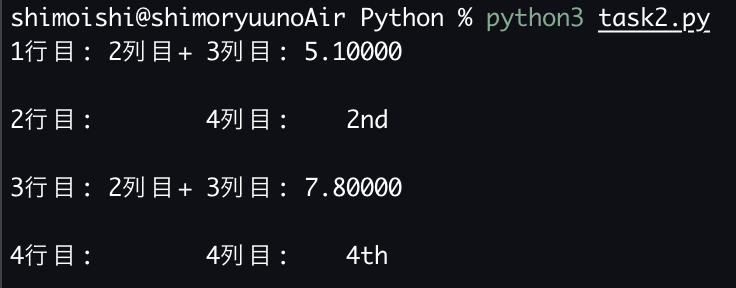
\includegraphics[width=0.8\linewidth]{Experiment_photo/task2.png}
    \caption{演習課題2の実行結果}
    \label{task2ans}
  \end{figure}
  演習課題2では,input.csvを1行ごと取り出してそれをさらに列ごとに配列の要素化している.配列にするときは
  ","区切りで分けた.行番号を2で割ったときに割り切れたときは偶数行,割り切れなかったときは奇数行として
  表示する形式を変更できるようにしている.

\subsection{演習課題3}
  \begin{screen}
    まずdata1.csvを保存し,data1.csvの1,2行目のコメント行をEditorなどで削除しなさい.
    このコメント行を削除したデータを読み込み,その3,8,10行目のみ,各行の1,2列目を表示するscriptを作成せよ.
    (Script例リスト7を参考にして,コメント行を削除せずに,その行を読み飛ばす処理を行っても良い.)
    さらに出力行を図13のようなリストで指定し,指定された行の1,2列目を表示するscriptを作成せよ.
    ただしリストloutputの要素数は3とは限らない.またlenを用いるとリストの要素数を取得することができる.
  \end{screen}
  この課題で作成したコードとその実行結果をそれぞれCode\ref{task3}と図\ref{task3ans}に示す.なお,Code\ref{data1.csv}
  を使用した.
  \lstinputlisting[caption=演習課題3, label=task3]{Python/task3.py}
  \begin{figure}[H]
    \centering
    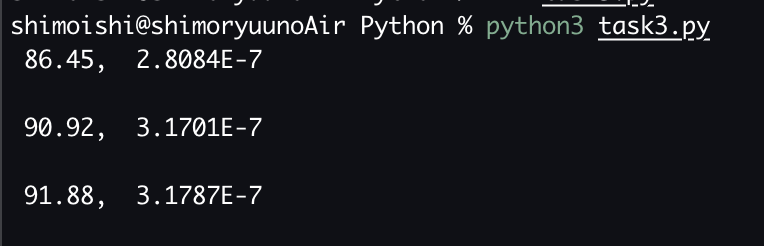
\includegraphics[width=0.8\linewidth]{Experiment_photo/task3.png}
    \caption{演習課題3の実行結果}
    \label{task3ans}
  \end{figure}

\subsection{演習課題4}
  \begin{screen}
    前の例題で用いたcsvファイルdata1.csvおよびそれと同じフォーマットのcsvファイルdata2.csv,csvファイルdata3.csvのそれぞれに対して,
    温度(1列目),抵抗率(2列目),電気抵抗(7列目),電気抵抗の測定誤差(8列目)を抜き出し,ファイルに出力するscriptを作成せよ.ただし,
    抵抗値が負のデータに関しては,先頭に"\#\#"を付けて出力すること.また出力ファイル名は適切に設定すること.
  \end{screen}
  この課題で作成したコードをCode\ref{task4}に示す.また,実行結果をCode\ref{d1.t},\ref{d2.t},\ref{d2.t}に示す.
  なお,Code\ref{data1.csv},\ref{data2.csv},\ref{data3.csv}を使用した.
  \lstinputlisting[caption=演習課題4, label=task4]{Python/task4.py}
  \lstinputlisting[caption=出力1, label=d1.t]{Python/data1.txt}
  \lstinputlisting[caption=出力2, label=d2.t]{Python/data2.txt}
  \lstinputlisting[caption=出力3, label=d3.t]{Python/data3.txt}

\subsection{研究課題}
  \begin{screen}
    data1.csv,data2.csv,data3.csvに対して,以下の条件を満たすようなscriptを作成せよ.
    \begin{itemize}
      \item 課題4のscriptで,matplotlibを使ってグラフを描画する.
      \item 横軸: 温度、縦軸: 電気抵抗値.
      \item 抵抗値の最大値・最小値に応じて、自動的に縦軸の範囲を指定.
      \item 最大値と最小値が二桁以上異なる場合は縦軸を対数グラフ.
      \item 画像(pngフォーマット)に保存.
    \end{itemize}
  \end{screen}
  研究課題で作成したコードをCode\ref{ex1}に示す.また,実行結果を図\ref{ex1p},\ref{ex2p},\ref{ex3p}にそれぞれ示す.
  なお,Code\ref{data1.csv},\ref{data2.csv},\ref{data3.csv}を使用した.
  \lstinputlisting[caption=研究課題, label=ex1]{Python/ex1.py}
  \begin{figure}[H]
    \centering
    \includegraphics[width=0.8\linewidth]{Python/data1.csv.png}
    \caption{data1.csvのグラフ}
    \label{ex1p}
  \end{figure}
  \begin{figure}[H]
    \centering
    \includegraphics[width=0.8\linewidth]{Python/data2.csv.png}
    \caption{data2.csvのグラフ}
    \label{ex2p}
  \end{figure}
  \begin{figure}[H]
    \centering
    \includegraphics[width=0.8\linewidth]{Python/data3.csv.png}
    \caption{data3.csvのグラフ}
    \label{ex3p}
  \end{figure}

\section{考察}
\subsection{演習課題1}
  

\subsection{演習課題2}
  

\subsection{演習課題3}




\end{document}